\chapter{Overlapping, heterogeneous age groups: atrial fibrillation}
\label{applications-age_groups}

Like many conditions analyzed in the GBD 2010 Study, Atrial
Fibrillation (AF) has no standard set of age groups for reporting.  The
meta-analysis of the data collected in systematic review must address
these heterogeneous age groups in some way. AF provides a prototypical
example of this, one where the implication of the modeling choices to
use an age-standardizing model can be compared to other possible
choices.  This chapter compares the estimates produced for AF
prevalence and incidence using an age-standardizing model to those
from a midpoint model.

AF is the most common type of cardiac arrhythmia.  Chaotic and
irregular heart rhythms originating in the atria cause poor blood flow
to the body.  The duration of AF episodes vary greatly.  First attacks
or paroxysmal AF are occasional, only lasting a few minutes or hours,
whereas persistent AF and permanent AF are chronic.  Symptoms include
heart palpitations, lack of energy, dizziness, shortness of breath and
chest discomfort, although some cases of atrial fibrillation are
symptomless.  AF may occur at any age with increasing risk for older
ages.  It is uncommon in children.  Other heart diseases tend to be
the underlying cause of AF.  AF is associated with with coronary heart
disease, hypertensive heart disease, valvular heart disease, heart
failure, cardiomyopathy, obesity and metabolic disorders such as
diabetes and hyperthyroidism. \cite{rich_epidemiology_2009,
  rho_asymptomatic_2005, fuster_acc/aha/esc_2006, radford_atrial_1977,
  TK_ref_from_Mehrdad}

The GBD 2010 Study defines AF as a patient having a least one episode
confirmed by a physician.  The systematic review of AF collected $3942$
data points, of which $247$ were from countries in Western Europe.  We
will consider only the Western European data in this chapter. It
consists of $20$ data points on disease incidence and $147$ on prevalence.
As seen from Figure \ref{fig:app-af data}, atrial fibrillation has
heterogeneous and overlapping age groups.  Without access to the
microdata needed to recreate homogeneous age groups, combining all of
this data must rely on age group modeling, as described in
Chapter~\ref{chap:age_group_model}.

    \begin{figure}[h]
        \begin{center}
            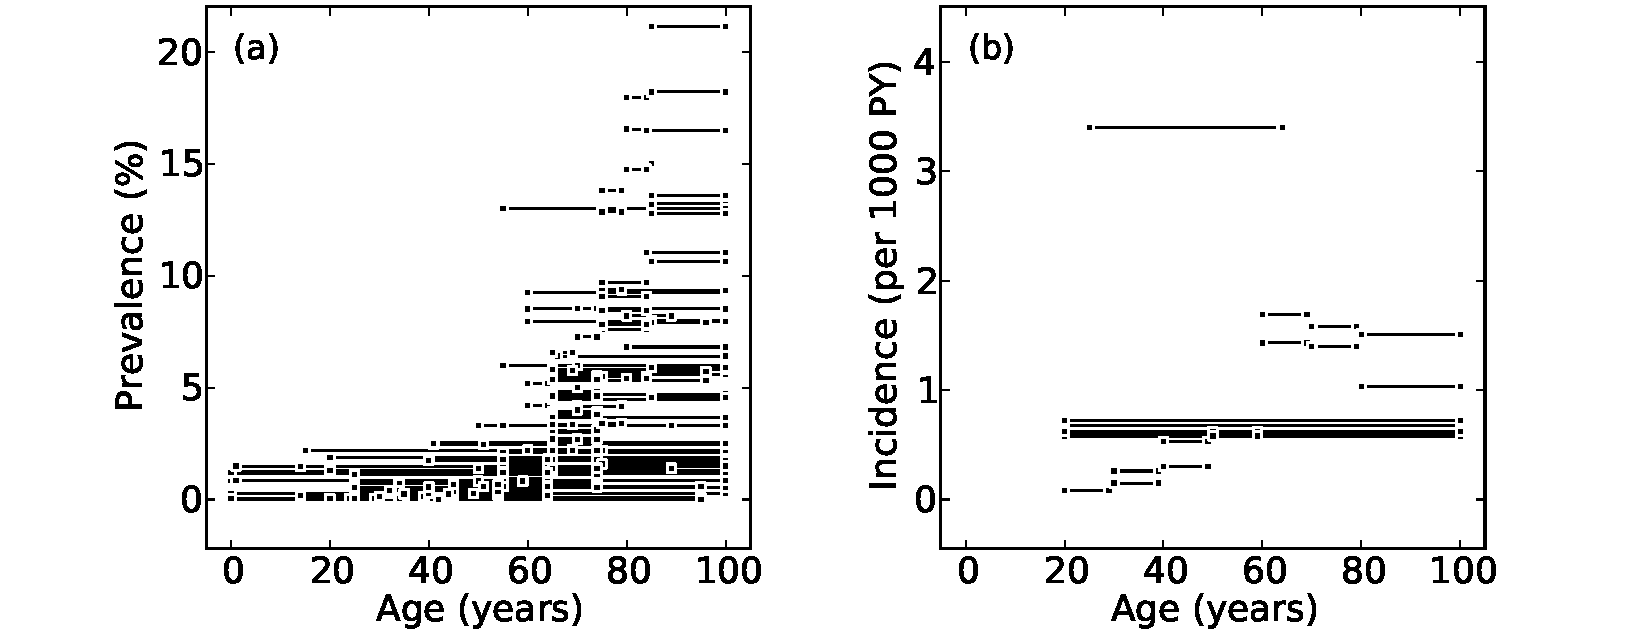
\includegraphics[width=\textwidth]{af-data.pdf}
            \caption{Data for Western Europe males with
              AF is an excellent example of heterogeneous
              and overlapping age groups.}
            \label{fig:app-af data}
        \end{center}
    \end{figure}

As discussed in Chapter \ref{theory-age_group_model-overlapping_data},
the simplest approach to modeling heterogeneous age groups is to apply
each age-specific rate measurement to the midpoint of the age interval.
Another solution to the heterogeneous age groups is to use age-standardizing.
Age-standardizing adds age weights to the age-specific rate according
to population structure.  The age-standardizing model uses a common
age pattern for all studies so that the age weights are the same for
all country-years, as discussed in more detail in Chapter
\ref{theory-age_group_model-overlapping_data}.

As the prevalence estimates in Figure \ref{fig:app-af srt p} show,
model choice changes the estimates. In estimates before age 80, the
differences are minimal, but in estimates for older ages, where the
data is sparser and noisier, the difference is substantial.

    \begin{figure}[h]
        \begin{center}
            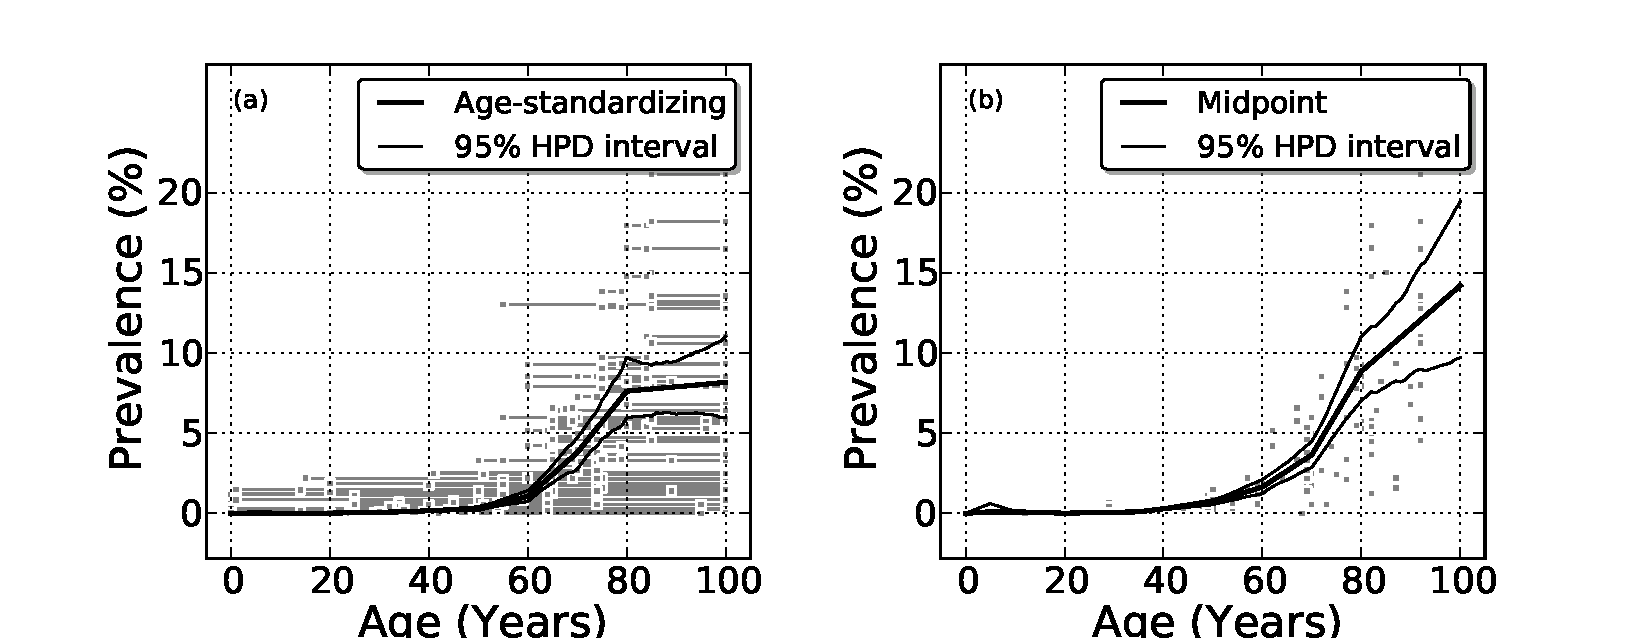
\includegraphics[width=\textwidth]{af-mp_v_hetero_srt_p.pdf}
            \caption{Comparison of prevalence of AF estimates for Western European
              males in 1990 using an age-standardizing
              or midpoint spline model.  Panel (a) shows the data and
              estimates for the age-standardizing model and panel (b)
              data and estimates for the midpoint model.}
            \label{fig:app-af srt p}
        \end{center}
    \end{figure}

Without additional information, one cannot say which model is preferred.
Further investigation with incidence does not provide much insight.  Like
the prevalence estimates, Figure \ref{fig:app-af srt i} shows that the
incidence estimates are similar in younger ages, but are different
in older ages.  The age-standardizing model does produce estimates with a
smoother age pattern.

    \begin{figure}[h]
        \begin{center}
            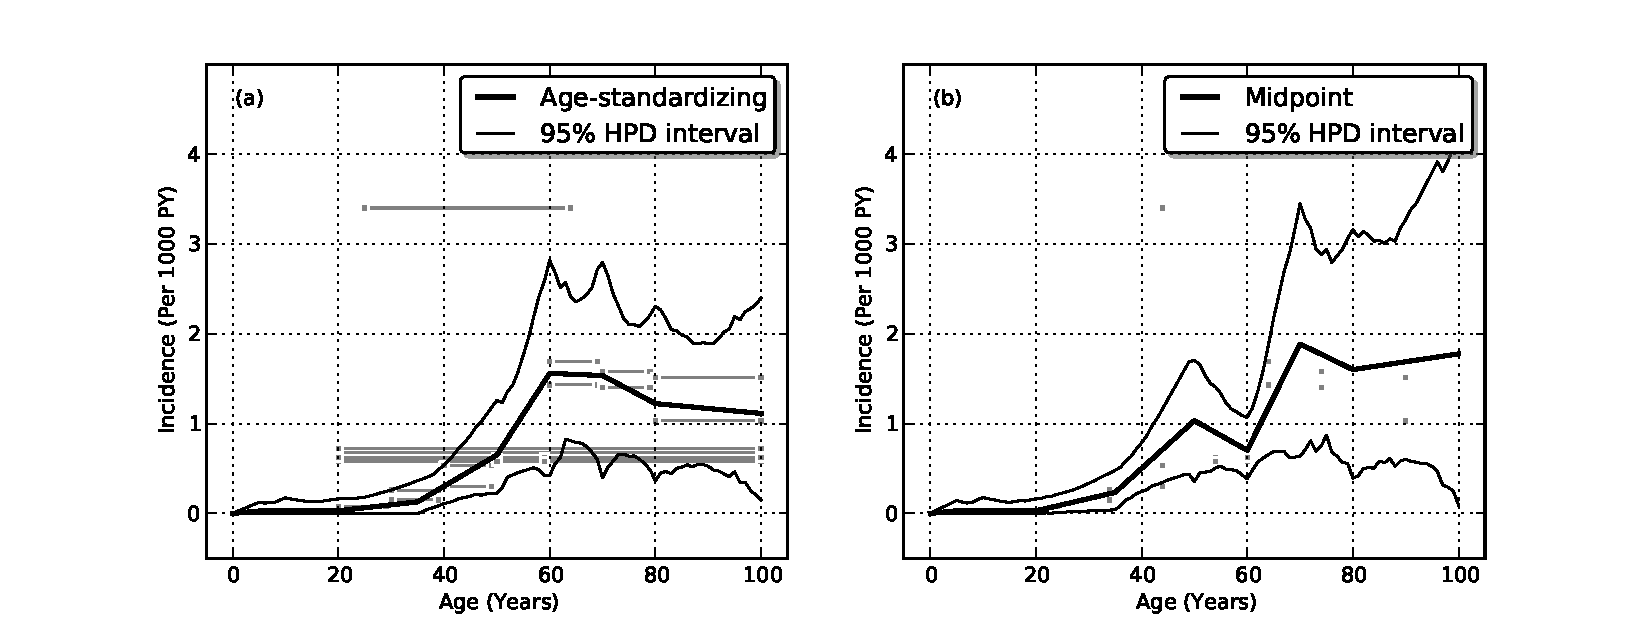
\includegraphics[width=\textwidth]{af-mp_v_hetero_srt_i.pdf}
            \caption{Comparison of incidence of AF estimates for Western European
              males in 1990 using (a) the age-standardizing spline model and (b)
              the midpoint spline model.}
            \label{fig:app-af srt i}
        \end{center}
    \end{figure}

Using all available data in a compartmental model, including the
limited available data on excess mortality, with-condition mortality
and cause-specific mortality, is a way to combine the data on
incidence and prevalence to produce consistent estimates of all
parameters simultaneously.  The prevalence estimates from this model
are preferred to a spline model of prevalence alone, because it
incorporates additoinal evidence.  Compartmental models are discussed in
more discussed in more detail in Chapters \ref{sys-dynamics}.  Figure
\ref{fig:app-af age-stand} shows consistent prevalence and incidence estimates
from the age-standardizing compartmental model.

The compartmental model estimates for incidence in Figure \ref{fig:app-af age-stand}
are very different from the spline model estimates.
Unlike the spline models, the compartmental model estimates for
incidence do not go through the data.  This is because the compartmental model
requires internal consistency, i.e. for every prevalent case there must be
a matching incident event.  The compartmental model shows that these levels
of prevalence cannot be achieved with the levels of incidence the data show.

    \begin{figure}[h]
        \begin{center}
            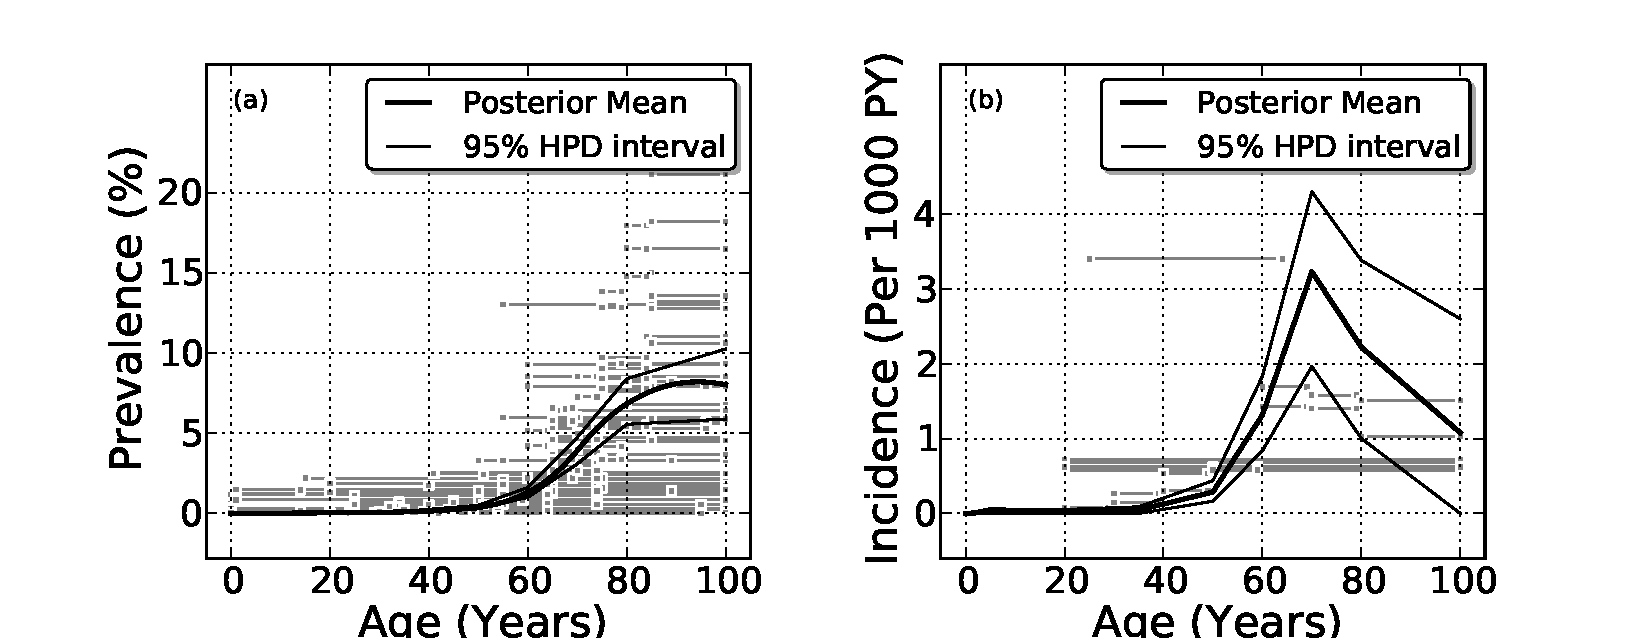
\includegraphics[width=\textwidth]{af-best_model.pdf}
            \caption{Estimates of prevalence (panel (a)) and incidence (panel (b))
              of AF in males in Western European in 1990 using
              an age-standardizing compartmental model.}
            \label{fig:app-af age-stand}
        \end{center}
    \end{figure}

Figure \ref{fig:app-af compare} compares the prevalence and incidence
estimates from the age-standardizing compartmental model to the
midpoint compartmental model.  Like the spline models, the
estimates only differ substantially in the oldest ages.

    \begin{figure}[h]
        \begin{center}
            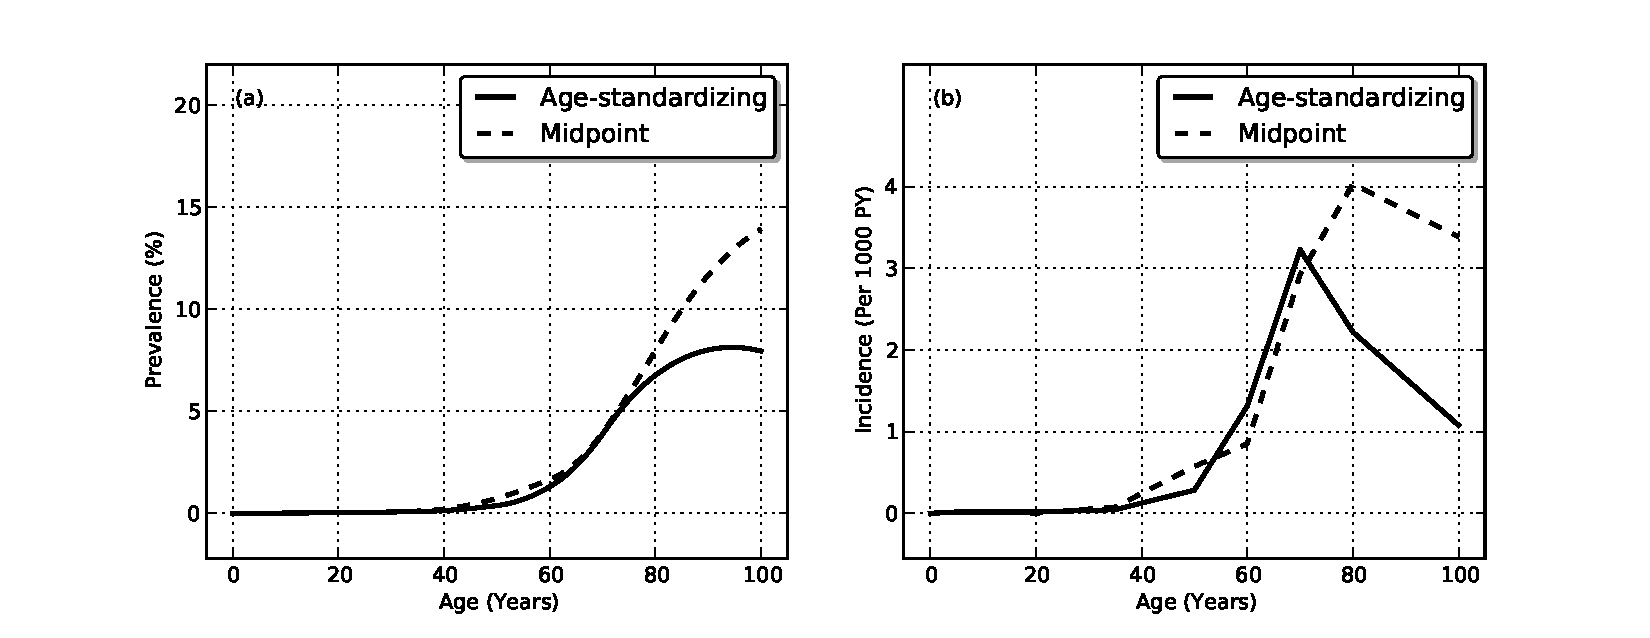
\includegraphics[width=\textwidth]{af-mp_v_hetero.pdf}
            \caption{A comparison of the estimated prevalence (panel (a)) and incidence
              (panel (a)) in Western European males with AF in 1990
              using an age-standardizing and midpoint compartmental models.}
            \label{fig:app-af compare}
        \end{center}
    \end{figure}

Choice of age group model has implications for disease estimates.
Estimated age pattern, trends and levels can differ between the
midpoint and age-standardizing models.  TK better conclusion.
